\documentclass{article}
\usepackage[utf8]{inputenc}
\usepackage{amsmath, dsfont, mathtools}
\usepackage{graphicx, float}
\usepackage[most]{tcolorbox}
\usepackage{enumitem}
\usepackage{hyperref}
\usepackage{tikz}
\usepackage{xcolor}

% ------------------------------------ %
%             Customization            %
% ------------------------------------ %

\usepackage[letterpaper, top=1in, left=1in, right=1in, bottom=1in]{geometry}
\setlength{\parindent}{0em}
\setlength{\parskip}{0.5em}
\setlist[enumerate]{itemsep=-0.5em} % Adjust the spacing as desired
\setlist[itemize]{itemsep=-0.5em} % Adjust the spacing as desired
\renewcommand{\baselinestretch}{1.25}

\title{MATH1853}
\author{Jax T}
\date{23 Dec}

\newtcolorbox{knBox}[2][]{
arc=2mm, 
lower separated=true, % Set to true to enable the separation between upper and lower sections
segmentation style={dashed, draw=black}, % Add dashed line style between the sections
fonttitle=\bfseries,
colbacktitle=white!10,
coltitle=black,
enhanced,
attach boxed title to top left={xshift=0.2cm,
        yshift=-2mm},
colframe=white!40!black,
boxrule=0.3mm,
colback=black!02,
title=#2,#1
}

\newtcolorbox{propBox}[2][]{
arc=2mm, 
lower separated=true, % Set to true to enable the separation between upper and lower sections
segmentation style={dashed, draw=black}, % Add dashed line style between the sections
fonttitle=\bfseries,
colbacktitle=green!10,
coltitle=black,
enhanced,
attach boxed title to top left={xshift=0.2cm,
        yshift=-2mm},
colframe=green!40!black,
boxrule=0.3mm,
colback=green!02,
title=#2,#1
}

\hypersetup{
    colorlinks=true,
    linkcolor=purple    % Color for internal links
}

\newenvironment{amatrix}[1]{%
  \left[\begin{array}{@{}*{#1}{c}|c@{}}
}{%
  \end{array}\right]
}

\newcommand{\note}[1]{\textcolor{gray}{\tiny #1}}

% ------------------------------------ %
%              Title page              %
% ------------------------------------ %
\begin{document}

\begin{titlepage}
    \null\vfill % Add vertical space to center the title and author
    
    \centering
    \Huge\textbf{MATH1853}
    
    \vspace{0.1cm}
    \Large\textbf{Notes Fall 2023}
    
    \vspace{1cm}
    \normalsize\textbf{Author:} Jax
    
    \normalsize\textbf{Contact:} enhanjax@connect.hku.hk
    \vfill % Add vertical space to center the remaining space
\end{titlepage}

% ------------------------------------ %
%               Document               %
% ------------------------------------ %

\section{Matrices}
Matrices are represented 
by captial letters: $A\in R^{r\times c}$.
$r \times c$ are the dimensions of a given matrix

\subsection{Basic operations}
\begin{knBox}[]{Addition}
    Matrices can perform per-element addition if their dimensions match.
    \tcblower
    $\begin{bsmallmatrix}
        1 & 2 & 3\\
        4 & 5 & 6
    \end{bsmallmatrix} + \begin{bsmallmatrix}
        6 & 5 & 4\\
        3 & 2 & 1
    \end{bsmallmatrix} = \begin{bsmallmatrix}
        7 & 7 & 7\\7 & 7 & 7
    \end{bsmallmatrix}
    $
\end{knBox}
\begin{knBox}[]{Scalar multiplication}
    Matrices can perform per-element multiplication with a scalar.
    \tcblower
    $\begin{bsmallmatrix}
        1 & 2 & 3\\3 & 2 & 1
    \end{bsmallmatrix} \times 2 = \begin{bsmallmatrix}
        2 & 4 & 6\\6 & 4 & 2
    \end{bsmallmatrix}$
\end{knBox}
\begin{knBox}[]{Matrix-matrix multiplication}
    Matrices can only multiply if their \underline{inner dimensions} match, otherwise there will be no solution.
    
    If a matrix is multiplied by another matrix, each \underline{element in the result matrix} is the sum of it's corresponding \underline{row in the original matrix} performing per-element multiplication on it's corresponding \underline{col in the applying matrix}

    \tcblower
    $\begin{bmatrix}
        1 & 2\\3 & 4
    \end{bmatrix} \times \begin{bmatrix}
        1 & 2\\3 & 4
    \end{bmatrix}=\begin{bmatrix}
        1\cdot 1 + 2 \cdot 3&1\cdot 2 + 2\cdot 4\\3\cdot 1 + 4\cdot 3&3\cdot 2 + 4\cdot 4
    \end{bmatrix} = \begin{bmatrix}
        7 & 10\\15 & 22
    \end{bmatrix}$
\end{knBox}
\begin{knBox}[]{Transposition}
    The function $A^T$ transposes the matrix $A$. It swaps the rows and columns of a matrix.
    \tcblower
    $\begin{bsmallmatrix}
        1&2\\3&4
    \end{bsmallmatrix}^T \equiv \begin{bsmallmatrix}
        1&3\\2&4
    \end{bsmallmatrix}\quad \begin{bsmallmatrix}
        1&2&3
    \end{bsmallmatrix}^T \equiv \begin{bsmallmatrix}
        1\\2\\3
    \end{bsmallmatrix}$
\end{knBox}

\subsection{Solving linear systems}
\begin{knBox}[]{Identity matrix}
    The identity matrix of $I\in \mathds{R}^{n\times n}$ with square dimensions is the matrix with diagonal elements of 1 and others 0.
    \tcblower
    $I\in \mathds{R}^{3\times 3}=\begin{bsmallmatrix}
        1&0&0\\0&1&0\\0&0&1
    \end{bsmallmatrix}$
\end{knBox}
\begin{knBox}[]{Row-echelon form}
    A matrix with a bottom-left or top-right triangle of 0's (excluding the diagonal) is considered to be in row-echelon form.
    \tcblower
    $\begin{bsmallmatrix}
        1&2&3\\0&1&2\\0&0&1
    \end{bsmallmatrix}\text{ and }\begin{bsmallmatrix}
        1&0&0\\1&2&0\\0&0&1
    \end{bsmallmatrix}$ are both considered in row-echelon form
\end{knBox}

\begin{knBox}[]{Augmented Matrix and Gaussian Elimination}
    Augmented matrices are an important tool to solve linear equations. The number of rows is equal to the number of variables in the equation. 

    GE are operations by \underline{rows}, performed on augmented matrices. The possible moves are:
    \begin{enumerate}
        \item Addition between rows ($R_1 + R_2$ adds row 2 to row 1, leaving row 2 unchanged)
        \item Multiplication of a row by a scalar ($\frac{1}{2}R_1$)
        \item Swapping rows ($R_1\leftrightarrow R_2$)
    \end{enumerate}
\end{knBox}

\subsubsection{Strict variables}
Consider the following linear system. We can take the coefficients and write it into AM form as followed:
\[
\begin{matrix}
    x_1 + 2x_2 = 3\\
    2x_1 + 5x_2 = 10
\end{matrix}\xRightarrow{\hspace{0.5cm}}
\begin{amatrix}{2}
    1 & 2 & 3 \\ \underbrace{2}_{x_1} & \underbrace{5}_{x_2} & 10
\end{amatrix}
\]

Then, we perform GE on the created augmented matrix to make the left side row-echelon.
\[
    \begin{amatrix}{2}
        1 & 2 & 3 \\ 2 & 5 & 10
    \end{amatrix} \xrightarrow{R_2-2R_1}
    \begin{amatrix}{2}
        1 & 2 & 3 \\ 0 & 1 & 4
    \end{amatrix}
\]
Deriving from the AM, we know:
\[
    \begin{matrix}
        x_1 + 2x_2 = 3\\
        x_2 = 4
    \end{matrix}
\]
So the solution is:
\[
    \begin{bmatrix}
        3-2\cdot 4\\
        4
    \end{bmatrix}\equiv
    \begin{bmatrix}
        -5\\
        4
    \end{bmatrix}
\]

\subsubsection{Inconsistent systems}
We say a system is inconsistent if a full row of 0 on the left is equal to a non-zero number. We can also conclude that there are no solutions to the system. The following is an example of a system with no solutions:
\[
\begin{matrix}
    x_1 + 2x_2 = 3\\
    2x_1 + 4x_2 = 10
\end{matrix}\xRightarrow{\hspace{0.5cm}}
\begin{amatrix}{2}
    1 & 2 & 3 \\ 2 & 4 & 10
\end{amatrix}\xrightarrow{R_2-2R_1}
\begin{amatrix}{2}
    1 & 2 & 3 \\ \mathcolor{red}{0 & 0 & 4}
\end{amatrix}
\]

\subsubsection{Free variable systems}
Free variables are variables with their corresponding columns having \textbf{no leading 1s} before 0s in the augmented matrix. If a system has free variables, the solution exists in a space, defined by the general solution.

Consider the following system with free variables, we can derive:
\[
    \begin{amatrix}{5}
        1 & 0 & \mathcolor{blue}{-5 & 0} & 8 & 3\\
        0 & 1 & \mathcolor{blue}{-4 & -1} & 0 & 6\\
        0 & 0 & \mathcolor{blue}{\underbrace{0}_{free} & \underbrace{0}_{free}} & 1 & 0
    \end{amatrix}\xRightarrow{\hspace{0.5cm}}\begin{matrix}
        x_1 -5x_3+8x_5 = 3\\
        x_2-4x_3-x_4=6\\
        x_5=0
    \end{matrix}\]
We can ignore the free variables, and substitute $x_5$ into both equations, deriving the general solution to be:
\[
    x=\begin{bmatrix}
        3+5x_3\\
        6+x_4+4x_3\\
        x_3\\
        x_4\\
        0
    \end{bmatrix}\]

\subsection{Matrix determinant}
Determinant is a property of a matrix, represented by $|A|$ or $det(A)$. Only square matrices have a determinant.
\subsubsection{Finding the value of determinant}
\begin{knBox}[]{$det(A\in \mathds{R}^{2\times 2})$}
    $for\quad A=\begin{bsmallmatrix}
        a&b\\c&d
    \end{bsmallmatrix},\quad |A| = ad - bc$
\end{knBox}
\begin{knBox}[]{$det(A\in \mathds{R}^{n\times n})$}
    Choose any row or column, then for each element, ignore their corresponding row and column to give the \emph{co-factor} of the element. 

    $det(A) = \sum(a\times det(\text{co-factor})\times (-1)^{r_a+c_a})$

    Where $a$ is an element from the picked row or column, and $r_a c_a$ are the row and column number of a

    \tcblower

    $|\begin{smallmatrix}1&2&3\\1&1&1\\3&2&1\end{smallmatrix}|=1|\begin{smallmatrix}
        1&1\\2&1
    \end{smallmatrix}|-2|\begin{smallmatrix}
        1&1\\3&1
    \end{smallmatrix}|+3|\begin{smallmatrix}
        1&1\\3&2
    \end{smallmatrix}|=0$

\end{knBox}
\begin{knBox}[]{Determinant of row-echelon form matrices}
    Product of diagonal elements.
    $|\begin{smallmatrix}
        1&2&3\\0&2&3\\0&0&3
    \end{smallmatrix}|=1\cdot 2\cdot 3=6$
\end{knBox}
\subsubsection{Determinant related properties}
\begin{enumerate}
    \item \hyperref[sec:dep]{Vector dependency}
    \item \hyperref[sec:inv]{Matrix inverse}
    \item \hyperref[sec:eigen]{Matrix eigenpairs}
\end{enumerate}


\subsection{Vectors}
Vectors are matrices with a single column, represented by letters with an arrow above them. $\overrightarrow{v} = \begin{bsmallmatrix}
    1\\2\\3
\end{bsmallmatrix}$

\begin{knBox}[]{Dot product}
    The dot product of two vectors $\vec{a}$ and $\vec{b}$ is essentially $\vec{a}^T\cdot\vec{b}$
\end{knBox}
\begin{knBox}[]{Vector length}
    $||\vec{v}||$ gives the length of a vector. $||\begin{bsmallmatrix}
        a&b&\dots
    \end{bsmallmatrix}^T||=\sqrt[]{a^2 + b^2 + \dots}$
\end{knBox}
\begin{knBox}[]{Unit vectors}
    They are vectors with the length of one. $\frac{\vec{v}}{||\vec{v}||}$ transforms the vector to a unit vector.
\end{knBox}
\begin{propBox}[]{Vector dependency}
    If $|\begin{smallmatrix}
        v_1 & v_2 & \dots
    \end{smallmatrix}|=0$, the vectors are dependent of each other
\end{propBox}
\label{sec:dep}
\begin{knBox}[]{Orthogonal projection}

    \begin{minipage}{0.6\textwidth}
        The \emph{orthogonal projection} of $a$ onto $b$ is $proj_ba = (\frac{a^Tb}{b^Tb})b$. 
    
        The component of $a$ perpendicular to $b$ is given by $a-proj_ba$
      \end{minipage}
      \hfill
      \begin{minipage}{0.35\textwidth}
        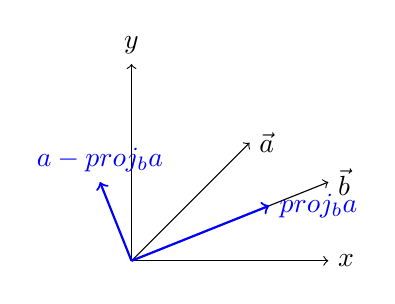
\begin{tikzpicture}[scale=0.5]
            % Axes
            \draw[->] (0,0) -- (5,0) node[right] {$x$};
            \draw[->] (0,0) -- (0,5) node[above] {$y$};
            
            % Vectors
            \draw[->] (0,0) -- (3,3) node[right] {$\vec{a}$};
            \draw[->] (0,0) -- (5,2) node[right] {$\vec{b}$};
            
            \draw[->, thick, blue] (0,0) -- (3.5 , 1.4) node[right] {$proj_ba$};
            \draw[->, thick, blue] (0,0) -- (-0.8 , 2) node[above] {$a - proj_ba$};
        \end{tikzpicture}
      \end{minipage}

\end{knBox}
\begin{propBox}[]{Orthonormal matrices}
    Orthonormal matrices have vector columns length 1, and which any product of two vectors is 0.
    For an orthonormal matrix $A$, $AA^T = I$
\end{propBox}
\begin{knBox}[]{Expressing a vector as a linear combination}
    We can express a vector $\vec{v}$ as the \emph{linear combination} of other vectors $a, b, \dots$ by:

    $v = proj_av + proj_bv + \dots$
\end{knBox}
\begin{knBox}[]{Vector spans}
    Vectors have the same span if they are \emph{linearly dependent}

    The dimension of $span(A)$ is given by the number of non-zero rows after GE 
\end{knBox}

\subsection{Matrix inverse}
\label{sec:inv}
Inverse is a property and function of a matrix, represented by $A^{-1}$
\begin{propBox}[]{Matrix inversibility}
    The matrix has an inverse if $|A|\ne 0$, and that it is a square matrix.
\end{propBox}
\begin{knBox}[]{$A^{-1} \in \mathds{R}^{2\times 2}$}
    $A^{-1} = \frac{1}{|A|}\begin{bmatrix}
        d &-b\\-c &a
    \end{bmatrix}$
\end{knBox}
\begin{knBox}[]{$A^{-1} \in \mathds{R}^{n\times n}$}
    $\begin{amatrix}{1}
        A&I
    \end{amatrix}\xrightarrow{GE}\begin{amatrix}{1}
        I&A^{-1}
    \end{amatrix}$
\end{knBox}

\subsection{Matrix eigenpairs}
\label{sec:eigen}
Matrices have properties \emph{eigenvalues} $\lambda_n$ and \emph{eigenvectors} $v_n$. They must satisfy the condition $Av=\lambda v$, and has the following properties:
\begin{enumerate}
    \item $\lambda_n$ and $v_n$ come in \emph{pairs} (each value correspond to a vector)
    \item Matrices can only have $\lambda_1, \lambda_2 \dots \lambda_n$ where $n$ is the smallest dimension of the matrix
    \item An $v_n$ includes all vectors of its multiple, and is non-zero
\end{enumerate}
By convention, $\lambda_1 > \lambda_2 > \dots > \lambda_n$
\begin{knBox}[]{Solving for eigenvalues}
    Note that we can rearrange the condition to $(A-I\lambda)v=0$, and into $|A-I\lambda| = 0$. Rearrange into polynomial equation and solve for $\lambda$ by first trial and error (if degree $> 2$) and then factorization.
    \tcblower
    The eigenvalues of $\begin{bsmallmatrix}
        1&1\\4&1
    \end{bsmallmatrix}$ can be found by $|\begin{smallmatrix}
        1-\lambda&1\\4&1-\lambda
    \end{smallmatrix}|=0:\quad(1-\lambda)^2 - 4 = 0\quad\rightarrow\quad\lambda_1=3,\ \lambda_2=-1$
\end{knBox}
\begin{propBox}[]{Algebratic and Geometric Multiplicity}
    \textbf{AM} is the number of times the value of $\lambda$ occur (e.g. $(1-\lambda)^2=0, \lambda_1=1$ has $AM=2$)

    \textbf{GM} is the size of nullspace (line of 0s) when plugging $\lambda$ into $(A-I\lambda)v=0$
\end{propBox}
\begin{knBox}[]{Solving for eigenvectors}
    Plug each $\lambda$ into $(A-I\lambda)v=0$, perform GE, then let the deterministic variable(s) as 1.
    \tcblower
    For $\lambda_1=3$ and $A=\begin{bsmallmatrix}
        1&1&1\\1&1&1\\1&1&1
    \end{bsmallmatrix}$:

    $(A-3\lambda)v=0 \xRightarrow{\hspace{0.5cm}} \begin{amatrix}{3}
        -2&1&1&0\\1&-2&1&0\\1&1&-2&0
    \end{amatrix}\xrightarrow{GE}\begin{amatrix}{3}
        -2&1&1&0\\0&-1&1&0\\\mathcolor{blue}{0&0&0&0}
    \end{amatrix}\begin{matrix}
        \ \\\ \\\mathcolor{blue}{GM=1}
    \end{matrix}$

    From the augmented matrix: $-2x_1+x_2+x_3=0,\quad -x_2+x_3=0$. 

    As $x_3$ is in both equations, let $x_3=1$: $x_2=1, x_1=1\rightarrow v_1=\begin{bsmallmatrix}
        1\\1\\1
    \end{bsmallmatrix}$
\end{knBox}
\begin{knBox}[]{Solving for eigenvectors with $GM\ 2$}
    Find the other eigenvector with $v = z_2 - proj_{z_1}z_2$
    \tcblower
    For $v=\begin{bsmallmatrix}
        -x_2-2x_3\\x_2\\x_3
    \end{bsmallmatrix}$, find the two solution forms as $z_1=\begin{bsmallmatrix}
        -1\\1\\0
    \end{bsmallmatrix},\ z_2\begin{bsmallmatrix}
        -2\\0\\1
    \end{bsmallmatrix}$

    Then let $z_1=v_1$, and solve for $v_2$ with $v_2=z_2-proj_{z_1}z_2=\begin{bsmallmatrix}
        -2\\0\\1
    \end{bsmallmatrix} - \frac{2+0+0}{1+1+0}\begin{bsmallmatrix}
        -1\\1\\0
    \end{bsmallmatrix}$
\end{knBox}

Related properties:

\begin{enumerate}
	\item \nameref{sec:diag}
	\item \nameref{sec:quad}
	\item \nameref{sec:diff}
\end{enumerate}

\subsection{Matrix diagonalization}
\label{sec:diag}
\begin{propBox}[]{Condition}
    A matrix can only be diagonalized if all of it's eigenpairs has their $AM = GM$.
\end{propBox}
\begin{knBox}[]{Eigendecomposition}
    $A=VDV^{-1},\quad\text{where }V=\begin{bmatrix}
        v_1\\\dots\\v_n
    \end{bmatrix},\ D=\begin{bmatrix}
        \lambda_1&0&0\\0&\ddots&0\\0&0&\lambda_n
    \end{bmatrix}$

    We can also derive $A^k=VD^kV^{-1}$
\end{knBox}

\subsection{Differential equations}
\label{sec:diff}
Given $x(0)$, solve for $x(t)$ with the following steps:
\begin{enumerate}
	\item Solve for eigenpairs
    \item $xk = cve^{\lambda t} + \dots + cve^{\lambda t}$
    \item Solve c by augmented matrix $\begin{amatrix}{3}
        v_1&\dots&v_n&x(0)
    \end{amatrix}$
\end{enumerate}

\subsection{Quadratic form}
\label{sec:quad}
A quadratic equation can be written into the form $Q(x)=xAx^T$, where $A$ is a symmetric matrix.
\begin{knBox}[]{Symmetric matrices}
    A matrix is symmetric if $A=A^T$
\end{knBox}
\begin{knBox}[]{Linear to matrix quadratic}
    \begin{flalign*}
        Q(x)&=ax_1^2+bx_2^2+cx_3^2+dx_1x_2+ex_2x_3+fx_1x_3\\
        &=\begin{bmatrix}
            x_1&x_2&x_3
        \end{bmatrix}\begin{bmatrix}
            a&d/2&f/2\\d/2&b&e/2\\f/2&e/2&c
        \end{bmatrix}\begin{bmatrix}
            x_1\\x_2\\x_3
        \end{bmatrix}
    \end{flalign*}
\end{knBox}
\begin{propBox}[]{Definitiveness of a quadratic}
    For $Q(x)=xAx^T$, considering the eigenvalues of $A$:
    \begin{itemize}
        \item $Q(x)$ is \emph{positive definitive} if $\forall\lambda > 0$
        \item $Q(x)$ is \emph{negative definitive} if $\forall\lambda < 0$
        \item $Q(x)$ is \emph{indefinite} if otherwise
        \item $Q(x)$ is \emph{p/n semi-definitive} if the conditions are inclusive (i.e. $\lambda \geq or \leq 0$)
    \end{itemize}

\end{propBox}
\begin{propBox}[]{Minimum and maximum values}
    $\lambda_{max} = max\{xAx^T:||x||=1\}$

    $\lambda_{min} = min\{xAx^T:||x||=1\}$

    Apply the corresponding $v\rightarrow x$ to find the min/max of $Q(x)$. Note that $||x||=1$ is a required restriction on $Q(x)$, otherwise its size would be infinite.
\end{propBox}


\section{Complex numbers}
The imaginary number $i=\sqrt{-1}$. A complex number is usually denoted as $z=a+bi$. In operations, the imaginary number can be considered as an unknown, though note that $i^2=-1$ (and so forth).
\subsection{Useful items}
\begin{propBox}[]{Common properties}
    The \emph{modulus}: $|z|=\sqrt{a^2+b^2}$

    The \emph{conjugate}: $conj(z) = \hat{z} = a-bi$

    The \emph{argument}: $arg(z) = \theta = 2tan^{-1}(\frac{b}{a+|z|})$
\end{propBox}

\begin{knBox}[]{Polar form}
    We can write a complex number in polar form: $z=r(\cos\theta+i\sin\theta),\quad \text{where } r=|z|$.

    This represents the point on a circle with radius $r$, at the angle $\theta$.
\end{knBox}

\begin{knBox}[]{Euler's formula}
    $re^{i\theta}=r(\cos\theta+i\sin\theta)$.

    Using the formula, we can easily derive:
    \begin{itemize}
        \item $(\cos\theta+i\sin\theta)^n = (\cos{n\theta}+i\sin{n\theta})$
        \item $(\cos\theta+i\sin\theta)^{-1} = (\cos{\theta}-i\sin{\theta})$
        \item $(\sin\theta+i\cos\theta) = i(\cos{\theta}-i\sin{\theta})=ie^{-i\theta}$
    \end{itemize}
\end{knBox}

\begin{propBox}[]{Complex roots}
    Consider $nz=k$, the solutions to the equation is:
    
    $\underbrace{kw^0 + kw^1 + \dots + kw^{n-1}}_{n\text{ solutions}}\quad for\ w = e^(\frac{2\pi i}{n})$, 
\end{propBox}

\begin{knBox}[]{Set notation}
    Elements in a set are \emph{unique}.
    \[A=\{\underbrace{\underbrace{1}_{\text{An element}},2,3}_{\text{Elements}}\}\quad\quad B=\{\underbrace{x}_{\text{For all}}\ |\ \underbrace{0<x<2}_{\text{Such that}}\underbrace{,}_{\text{And}}\quad x\in\mathds{R}\}=\{1\}\]
\end{knBox}

\subsection{Image under complex function}
Given a complex function $f(z)$ and a set of complex numbers $D=\{g(z)\in \mathds{C}:h(z)\}$, our goal is to solve for the function $f(D)$ in a form that we can identify the shape / image.

\subsubsection{General steps}
\begin{enumerate}
    \item Find $f(D)$ by finding $f(g(z))$
    \item Let $f(g(z))$ be $x'+y'i$, then solve for $x$ and $y$ in terms of $x'$ and $y'$ \\(Note that $g(z)$ and $h(z)$ are functions of $x+yi$)
    \item Substitute your $x$ and $y$ to $f(D)$, so that all unknowns are in terms of $x'$ and $y'$
    \item Rearrange $h(z)$ to solve the shape of the image
\end{enumerate}

\subsubsection{Simple example}
Let $D=\{x+iy \in \mathds{C}\ | |x+iy|>1\}$, with complex function $f(z)=-1/z$. Find $f(D)$, then sketch the picture of $f(D)$ on the complex plane. \note{23 Dec, Part 2 Assignment 2 Question 3}

\begin{center}
We first find $f(D)$ by finding $f(x+yi)$:
\[f(x+yi)=\frac{-1}{x+yi}\rightarrow f(D)=\{\frac{-1}{x+yi}\in \mathds{C}||x+yi|>1\}\]
Then let $\frac{-1}{x+yi}$ be $x'+y'i$, then solve for $x$ and $y$ in terms of $x'$ and $y'$
\[x'+y'i=\frac{-1}{x+yi}\rightarrow x+yi=\frac{-1}{x'+y'i}\]
Substitute the values we found into $f(D)$
\[f(D)=\{x'+y'i\in \mathds{C}||\frac{-1}{x'+y'i}|>1\}\]
Then finally we rearrange the right side of the equation as:
\[\frac{1}{\sqrt{x'^2+y'^2}}>1\]
\[1>x'^2+y'^2\]
Therefore, we can conclude that the image is a filled circle with radius 1 (excluding edges):

    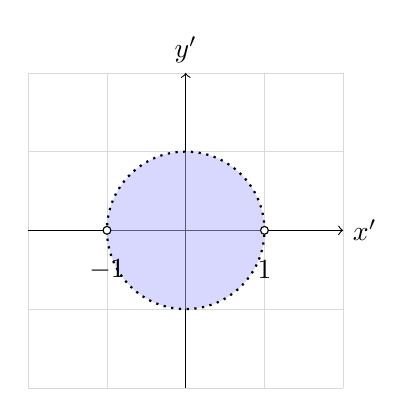
\begin{tikzpicture}
        % Grid
        \draw[help lines, color=gray!30] (-2,-2) grid (2,2);
        
        % Axes
        \draw[->] (-2,0) -- (2,0) node[right] {$x'$};
        \draw[->] (0,-2) -- (0,2) node[above] {$y'$};
        
        % Filled circle
        \fill[blue!30,opacity=0.5] (0,0) circle (1);
        
        % Dotted circle edges
        \draw[dotted,thick] (0,0) circle (1);
        
        % Labels
        \node[fill=white,draw=black,circle,inner sep=1pt] at (1,0) {};
        \node at (1,-0.5) {$1$};
        \node[fill=white,draw=black,circle,inner sep=1pt] at (-1,0) {};
        \node at (-1,-0.5) {$-1$};
        
      \end{tikzpicture}
\end{center}

\subsubsection{A more elegant way}
We can use Euler's formula to solve questions involving circles. Using the above example:
\begin{center}
    We let $x+yi$ as $re^{i\theta}$ and substitute:
    \[D=\{re^{i\theta}\in\mathds{C}|\underbrace{r>1}_{\text{As $|z|$ is $r$}}\}\]
    Then following the usual steps:
    \[f(D)=\{-r^{-1}e^{-i\theta}\in \mathds{C}| r > 1\}\]
    \[f(D)=\{r^{-1}\underbrace{e^{-i\theta+i\pi}}_{-1=e^{i\pi}}\in \mathds{C}| r > 1\}\]
    \[Let\ r'=r^{-1}, \theta'=\pi-\theta\rightarrow r=r'^{-1}\]
    \[f(D)=\{r'e^{i\theta'}\in \mathds{C}| r^{-1} > 1\}\]
    \[f(D)=\{r'e^{i\theta'}\in \mathds{C}| r < 1\}\]
\end{center}

\section{Hyperbolic functions}
The scope of this course only focuses on these three functions:
\[\sinh x=\frac{e^{ix}+e^{-ix}}{2}\quad\quad\cosh x=\frac{e^{ix}-e^{-ix}}{2}\quad\quad\tanh x=\frac{\sinh x}{\cosh x}\]

\section{Probabilities}
\begin{knBox}[]{Combinations}
    The formula for combinations, also known as the binomial coefficient, is given by:
    
    \[
    \binom{n}{r} = \frac{n!}{r!(n-r)!}
    \]
    
    Which represents the number of ways to choose r items from a set of n distinct items without regard to their order.
\end{knBox}

\begin{propBox}[]{Pascal's rule}
    Pascal's rule is given by $\binom{n+1}{r}=\binom{n}{r}+\binom{n}{r-1}$
\end{propBox}
Probability measures the likelihood of an event happening. It assigns a numerical value between 0 and 1 to an event, where 0 represents an impossible event and 1 indicates a certain event.\\For example, the probability of flipping a fair coin and getting heads is 0.5, as there are two equally likely outcomes (heads or tails).\\The key to understanding probabilities (or anything else) is practice.

\subsection{Infinite sets}
\begin{table}[ht]
    \begin{tabular}{|c|l|l|}
    \hline
    \textbf{Set} & \textbf{Description} & \textbf{Example} \\
    \hline
    $\mathds{Z}$ & Integers & $-1,0,1$\\
    \hline
    $\mathds{N}$ & Natural & $0,1,2$\\
    \hline
    $\mathds{R}$ & Real & Any number $\frac{4}{7}, 0.1, 1, \pi$\\
    \hline
    $\mathds{Q}$ & Rational & Any number that can be expressed as a fraction $\frac{22}{7}$\\
    \hline
    $\mathds{C}$ & Complex & $a+bi$ \\
    \hline
    \end{tabular}
\end{table}

\subsection{Venn diagrams}
\begin{minipage}{0.65\textwidth}
    Venn diagrams illustrate concepts like intersections, unions, which is a good way to visualize probabilities. The overlapping regions indicate elements that belong to multiple sets, while non-overlapping regions represent elements unique to specific sets. 

    In this example, two circles are drawn to represent sets A and B. The overlapping region is labeled as the intersection of sets A and B, denoted by A $\cap$ B.
\end{minipage}
\hfill
\begin{minipage}{0.3\textwidth}
    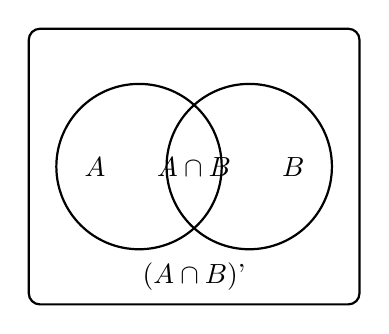
\begin{tikzpicture}[scale=0.7]
        \draw[thick, rounded corners] (-2,-2.5) rectangle (4,2.5);
        \draw[thick] (0,0) circle (1.5);
        \draw[thick] (2,0) circle (1.5);
        \node at (-0.8,0) {$A$};
        \node at (2.8,0) {$B$};
        \node at (1,0) {$A \cap B$};
        \node at (1,-2) {($A \cap B$)'};
    \end{tikzpicture}
\end{minipage}

\subsection{Probability notation and event types}
\begin{center}
    \begin{table}[H]
        \begin{tabular}{|c|c|c|}
        \hline
        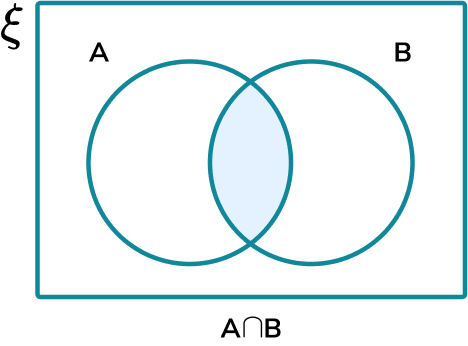
\includegraphics[width=5cm]{IMG/AND.png} & 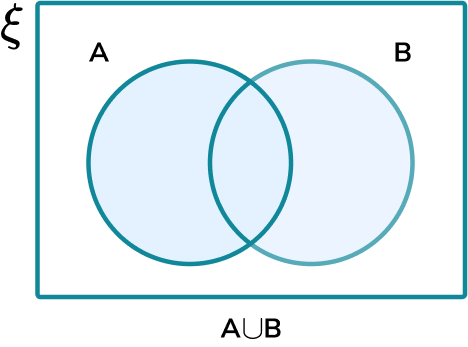
\includegraphics[width=5cm]{IMG/OR.png} & 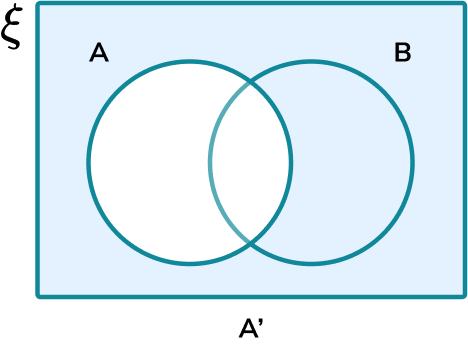
\includegraphics[width=5cm]{IMG/NOT.png} \\
        \hline
        A and B & A or B & Not A\\
        \hline
        Intersection & Union & Compliment\\
        \hline
        \end{tabular}
    \end{table}
\end{center}
\begin{propBox}[]{Conditional probabilities}
    The probability of A given that B occurs: $P(A\ |\ B) = \frac{P(A\cup B)}{P(B)}$
\end{propBox}

\begin{propBox}[]{Independent events}
    A and B are said to be \emph{independent} if $P(A) \times P(B) = P(A\cap B)$.

    Being independent means that the probability of an event \emph{has no influence on the other}
\end{propBox}

\subsection{Random variables}
\begin{knBox}[]{Notation}
    Random variables are denoted with capital letters $X$\\
    The possible outcomes are denoted with regular letters $x$\\
    Probability that the outcome of $X$ is $x$ is denoted by $P(X=x)$
\end{knBox}
\begin{propBox}[]{Expected value and Variance}
    $E(X^n)=\sum(x^n\cdot P(X=x))$ gives the expected value, which represents the mean value (outcome) of the random variable.

    $Var(X)=E(X^2)-E(X)^2$ gives the variance, which is a measure of the variability of the random variable's outcomes.
\end{propBox}
\begin{propBox}[]{Operations of $E(X)$ and $Var(X)$}
    $E(X+Y)=E(X)+E(Y)$, which any addition / subtraction function within $E()$ can be expanded.\\
    \\
    If $X$ and $Y$ are independent:
    $Var(X+Y) = Var(X) + Var(Y),\quad\quad E(XY)    = E(X)\cdot E(Y)$\\
    \\
    $for\ Y=aX+b:$ $E(Y)=aE(X)+b,\quad\quad Var(Y)=a^2Var(X)$

\end{propBox}

\subsection{Joint random variables}
Joint random variables are in the form $P(X=x, Y=y)$. We can visualize the joint distribution in the following way:
\begin{center}
    \begin{table}[H]
        \begin{tabular}{|c|c|c|c|}
            \hline
            $X \symbol{92}Y$ & $x_1$ & $x_2$ & \\
            \hline
            $y_1$ & $P(X=x_1, Y=y_1)$ & $P(X=x_2, Y=y_1)$ & $P(Y=y_1)$\\
            \hline
            $y_2$ & $P(X=x_1, Y=y_2)$ & $P(X=x_2, Y=y_2)$ & $P(Y=y_2)$\\
            \hline
             & $P(X=x_1)$ & $P(X=x_2)$ & \\
            \hline
        \end{tabular}
    \end{table}
    \vspace{-1cm}
\end{center}
Note that the sum of a column or row results in the corresponding variable's probability of outcome.

\begin{propBox}[]{Expected value}
    $E(X+Y)   = \sum((x+y) P(X=x, Y=y))$\\
    $E((XY)^n) = \sum((xy)^n P(X=x, Y=y))$
\end{propBox}

\subsection{Random variables of random variables (outcomes)}
For random variables modelled in the following way:
\[\bar{X}=X_1+X_2+\dots+X_n\]
We can deduce that:
\[E(\bar{X})=\frac{E(X_1)+\dots+E(X_n)}{n}=\frac{nE(X)}{n}\]
\[Var(\bar{X})=\frac{Var(X_1)+\dots+Var(X_n)}{n^2}=\frac{nVar(X)}{n^2}\]

\begin{propBox}[]{Expected value and Variance}
    $E(\bar{X})   = E(X)$\\
    $Var(\bar{X}) = \frac{Var(X)}{n}$
\end{propBox}

\section{Probability distributions}
A \emph{continuous} random variable has probabilities the area under its curve. Hence, $P(X=n)$ for any outcome $n$ is $0$. A \emph{discrete} random variables have specific probabilities assigned to an outcome.\\
\\
\begin{minipage}{0.45\textwidth}
    \begin{knBox}[]{Operation on continous ranges}
        $P(X<x)=P(X\leq x)$\\
        $P(X>x)=1 - P(X<x)$\\
        $P(a\leq X\leq b)=P(X<b)-P(X<a)$
    \end{knBox}
\end{minipage}
\hfill 
\begin{minipage}{0.45\textwidth}
    \begin{knBox}[]{Operation on discrete ranges}
        $P(X<x)=P(X\leq x-1)$\\
        $P(X>x)=1-P(X\leq x)$\\
        $P(a\leq X\leq b)=P(X\leq b)-P(X\leq a-1)$
    \end{knBox}
\end{minipage}
\subsection{Probability distribution functions}
A \emph{p.d.f} is a continuous function that returns the probability of the given outcome. The following is an example of a p.d.f:
\[
X\sim f(x) = \begin{cases} 
Kx^2 & 0 \leq x \leq 1 \\
0 & \text{otherwise}
\end{cases}
\]
\begin{propBox}[]{Using the function}
    $P(X=x)=0$\\
    $P(a<X<b)=P(a\leq X\leq b)=\int_{a}^{b}f(x)dx$\\
    \\
    Note that $\int_{\infty}^{-\infty}f(x)dx = 1$, as the total probability of any event is 1. This condition \emph{must be true} for $f(x)$ to be a valid p.d.f. Hence for the example $K=3$
\end{propBox}
\begin{propBox}[]{Expected value}
    $E(X^n)=\int_{\infty}^{-\infty}x^nf(x)dx$
\end{propBox}
\subsection{Cumulative distribution function}
To obtain a \emph{c.d.f} $X'\sim F(x)$where $P(X'=x) = P(X < x)$, all we have to do is integrate the p.d.f: 
\[F(X)=\int f(x)dx\]
Using our example:
\[F(X)=\begin{cases}
    1 & x > 1\\
    x^3 & 0 < x < 1\\
    0 & x < 0\\
\end{cases}\]
And to convert a c.d.f back to it's p.d.f, all we have to do is differentiate $F(x)$:
\[f(x)=\frac{d}{dx}F(x)\]

\subsection{Statistical distributions}
\subsubsection{Common statistical distribution}
\begin{tabular}{|l|l|l|l|l|l|}
    \hline
    &&&&&\\
    \note{Continuous}&\note{Discrete}&\note{Discrete}&\note{Discrete}&\note{Discrete}&\note{Discrete}\\
    \underline{Expo}nential     & \underline{Ber}noulli     & \underline{B}inomial        & \underline{Geo}metric   & \underline{N}egative \underline{B}inomial & \underline{Po}ssion\\
    $Expo(\lambda)$             & $Ber(p)$                  & $B(n, p)$                   & $Geo(p)$                & $NB(n, p)$                                & $Po(\lambda)$ \\
    $\lambda e^{-\lambda x}$    & $p$ if true, else $(1-p)$ & $\binom{n}{x} p^x(1-p)^{n-x}$  & $p(1-p)^{x-1}$       & $\binom{x-1}{n-1} p^n(1-p)^{x-n}$         & $\frac{\lambda^x}{x!} e^{-\lambda}$ \\
    $E=\lambda^{-1}$            & $E=p$                     & $E=np$                      & $E=\frac{1}{p}$         & $E=\frac{n}{p}$                           & $E=\lambda$ \\
    $Var=\lambda^{-2}$          & $Var=p(1-p)$              & $Var=np(1-p)$               & $Var=\frac{1-p}{p2}$    & $Var=\frac{n(1-p)}{p2}$                   & $Var=\lambda$ \\
    &&&&&\\
    \hline
\end{tabular}
\subsubsection{Usage cases}
\vspace{-0.2cm}
\begin{itemize}
    \item Ber: Outcomes only $True$ or $False$
    \item B: $x$ successes in $n$
    \item Geo: $1$st success at $x$ tries
    \item NB: $n$th success at $x$ tries
    \item Po: $x$ successes in interval $\lambda$
\end{itemize}

\subsubsection{Normal distribution}
The \underline{N}ormal distribution is given by the following formula (which you don't have to memorize):
\[X\sim N(\mu, \sigma^2)=\frac{1}{\sqrt{2\pi\sigma^2}} e^{-\frac{(x-\mu)^2}{2\sigma^2}},\quad\quad\text{where }\underbrace{\mu}_{\text{mean}},\underbrace{\sigma^2}_{\text{variance}}\]
To calculate $P(X<x)$, we have to \emph{standardize} our $N$ by $Z\sim N(0, 1)$, $P(X<x)=P(Z<\frac{x-\mu}{\sigma})$. Here $Z$ is the \emph{standard normal variable}.

\begin{knBox}[]{Reading the Z-table}
    For $P(Z<z)=p$, to find $p$, locate the header and leftmost column in the z-table such that their \emph{sum} is $z$. The corresponding intersecting cell is $p$.\\
    $Z_p$ gives the value $z$ in $P(Z<z)=p$
\end{knBox}
\begin{propBox}[]{Critical interval}
    The critical interval is given by:
    \[C.I.=[\bar{X}\pm Z_{\frac{C.L.+1}{2}}\times\frac{\sigma}{\sqrt{n}}],\quad\quad\text{where }\underbrace{C.L.}_{\text{Confidence level}},\ \underbrace{\bar{X}}_{\text{Mean value}}\]
    Hence, we can derive that the critical interval width is:
    \[2\times Z_{\frac{C.L.+1}{2}}\times\frac{\sigma}{\sqrt{n}}\]
\end{propBox}

\end{document}